%\subsection{Выгрузка данных}
%%\marginnote{\Date{Вт.}{07}{Апр.}{2017}}[-40pt]
%\begin{itemize}	
%	\item В «Рознице» открываем обработку «V8Exchan83.epf»
%	Рис.~\ref{ris:4.jpg}	
%	\begin{figure}[H]
%		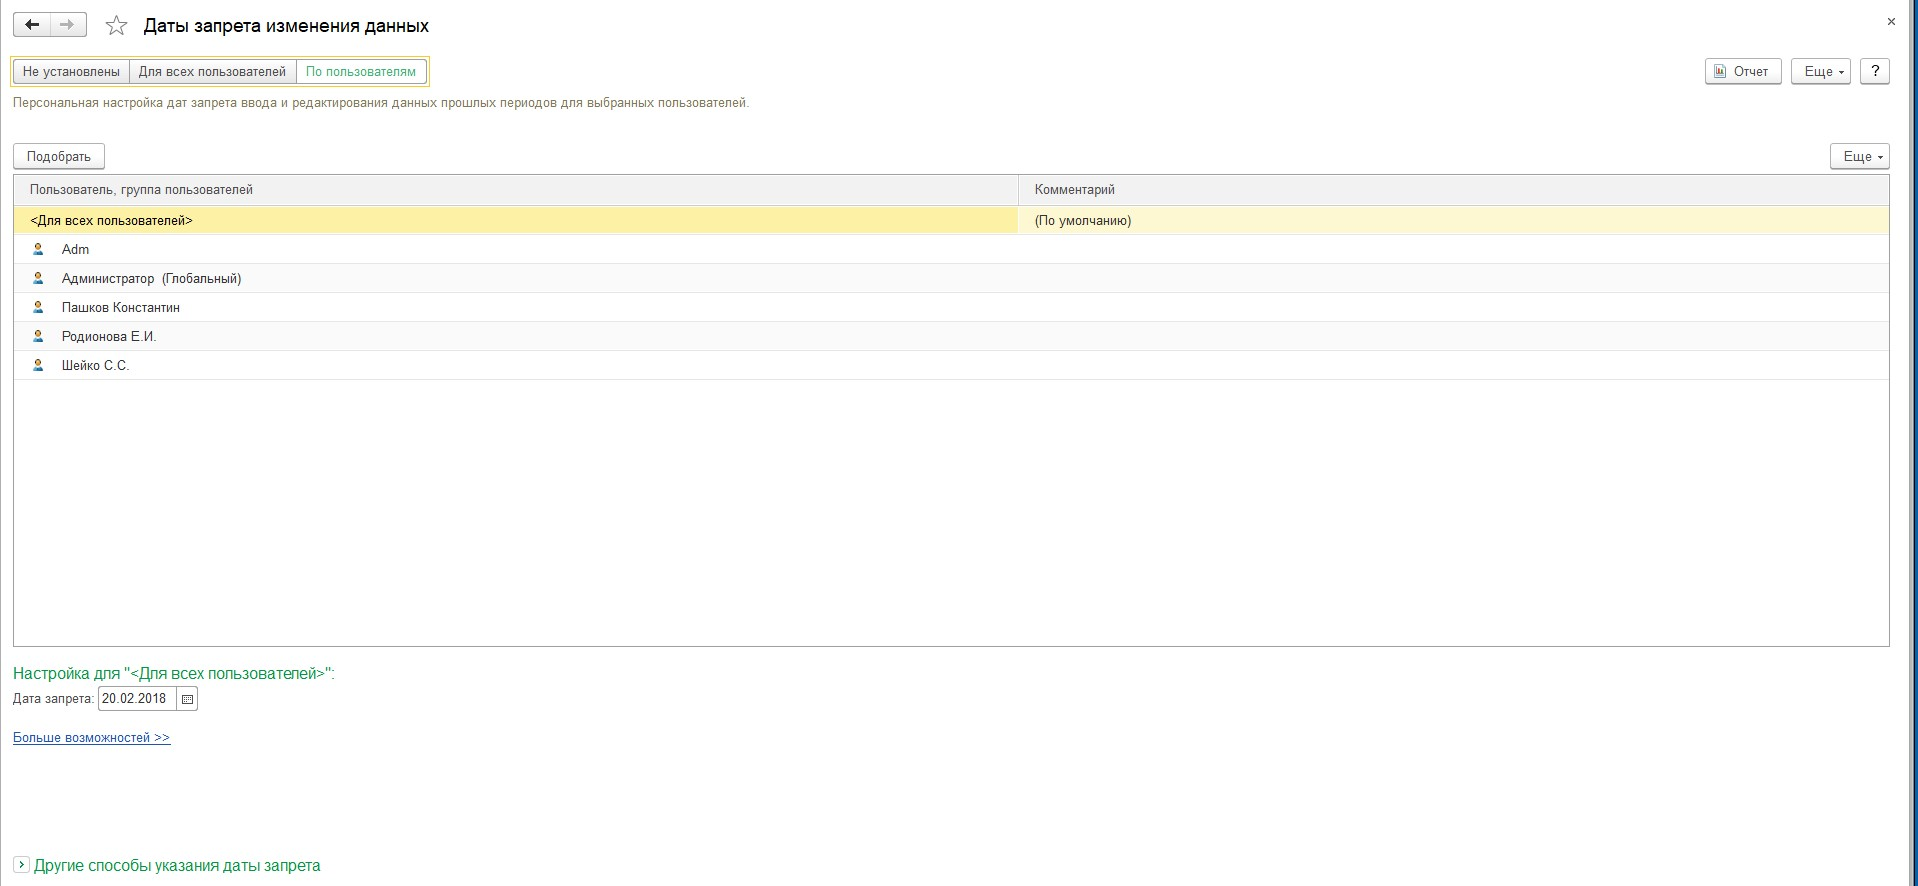
\includegraphics[width=0.8\textwidth]{4.jpg}
%		\caption{Обработка выгрузки данных из "<1С Розница">.}
%		\label{ris:4.jpg}
%	\end{figure}
%	
%	\item	Выбираем файл с правилами выгрузки «ПравилаОбменаДанными.xml» в "Имя файла правил на сервере".
%%	\item Когда все цены заполнены документ можно провести \par используя кнопку 
\includegraphics[width=0.02\linewidth]{images/pr} ,,провести'' или \keys{Провести и закрыть}.
%	\item После загрузки правил снимаем галочки со всех пунктов в дереве объектов
%	Рис.~\ref{ris:5.jpg}	
%	\begin{figure}[H]
%		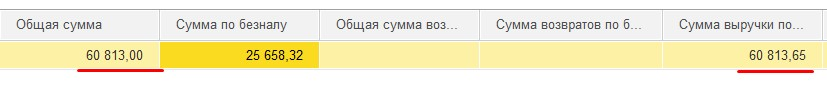
\includegraphics[width=0.8\textwidth]{5.jpg}
%		\caption{Загруженные правила.}
%		\label{ris:5.jpg}
%	\end{figure}
%Перед началом выгрузки необходимо заполнить нужные параметры:
%\item Период выгрузки (указываем весь месяц)
%\item На вкладке "<Параметры выгрузки"> заполняются два параметра:
%\subitem ДатаВыгрузкаОстатков (последним днем периода выгрузки) 
%\subitem КомплектующиеКулинарии (группой «Комплектующие» из справочника «Номенклатура»)
%Оба параметра будут использованы для выгрузки себестоимости комплектующих
%	Рис.~\ref{ris:6.jpg}
%	\begin{figure}[H]
%		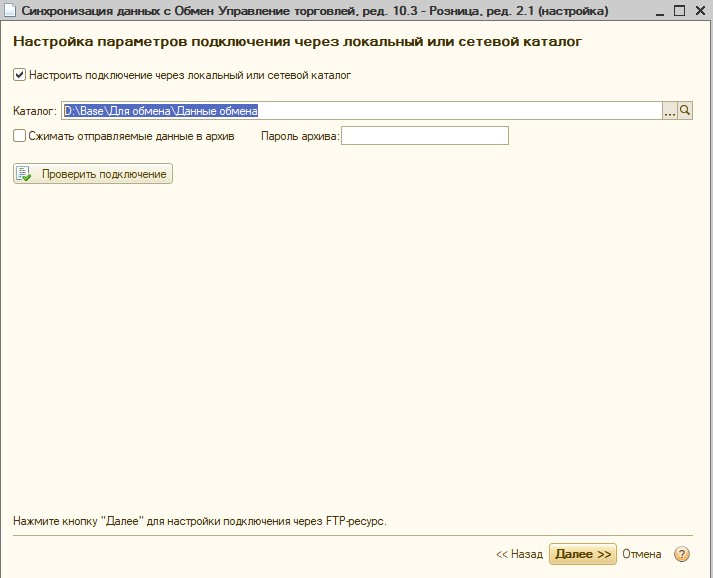
\includegraphics[width=0.46\textwidth]{6.jpg}
%		\caption{Парметры.}
%		\label{ris:6.jpg}
%	\end{figure}
%Для упрощения выгрузки-загрузки на данном этапе и получения более полного контроля над процессом, каждый объект будем выгружать в отдельный файл. Объекты из ветки "<Удаленные"> не выгружаем.\par Выгружать данные можно в любой последовательности, порядок загрузки будет указан ниже. 
%\item Выбираем элемент для выгрузки
%\item Выбираем файл куда будем выгружать
%\item Нажимаем \keys{Выгрузить данные}.
%	Рис.~\ref{ris:7.jpg}
%	\begin{figure}[H]
%		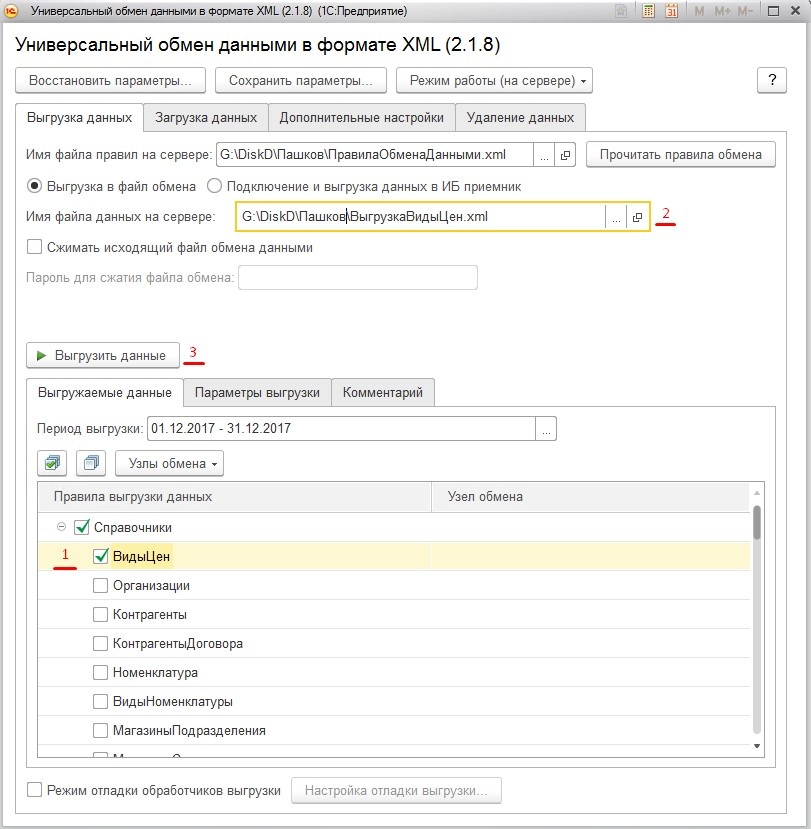
\includegraphics[width=0.46\textwidth]{7.jpg}
%		\caption{Выгрузка объекта.}
%		\label{ris:7.jpg}
%	\end{figure}
%Повторяем эту последовательность для всех нужных объектов, не забывая указывать новый файл для выгрузки. \par
%Когда все данные выгружены, запускаем "<УТ"> и приступаем к загрузке.
%
%\end{itemize}
